\begin{figure}
	\centering
	\begin{subfigure}[b]{.58\textwidth}
		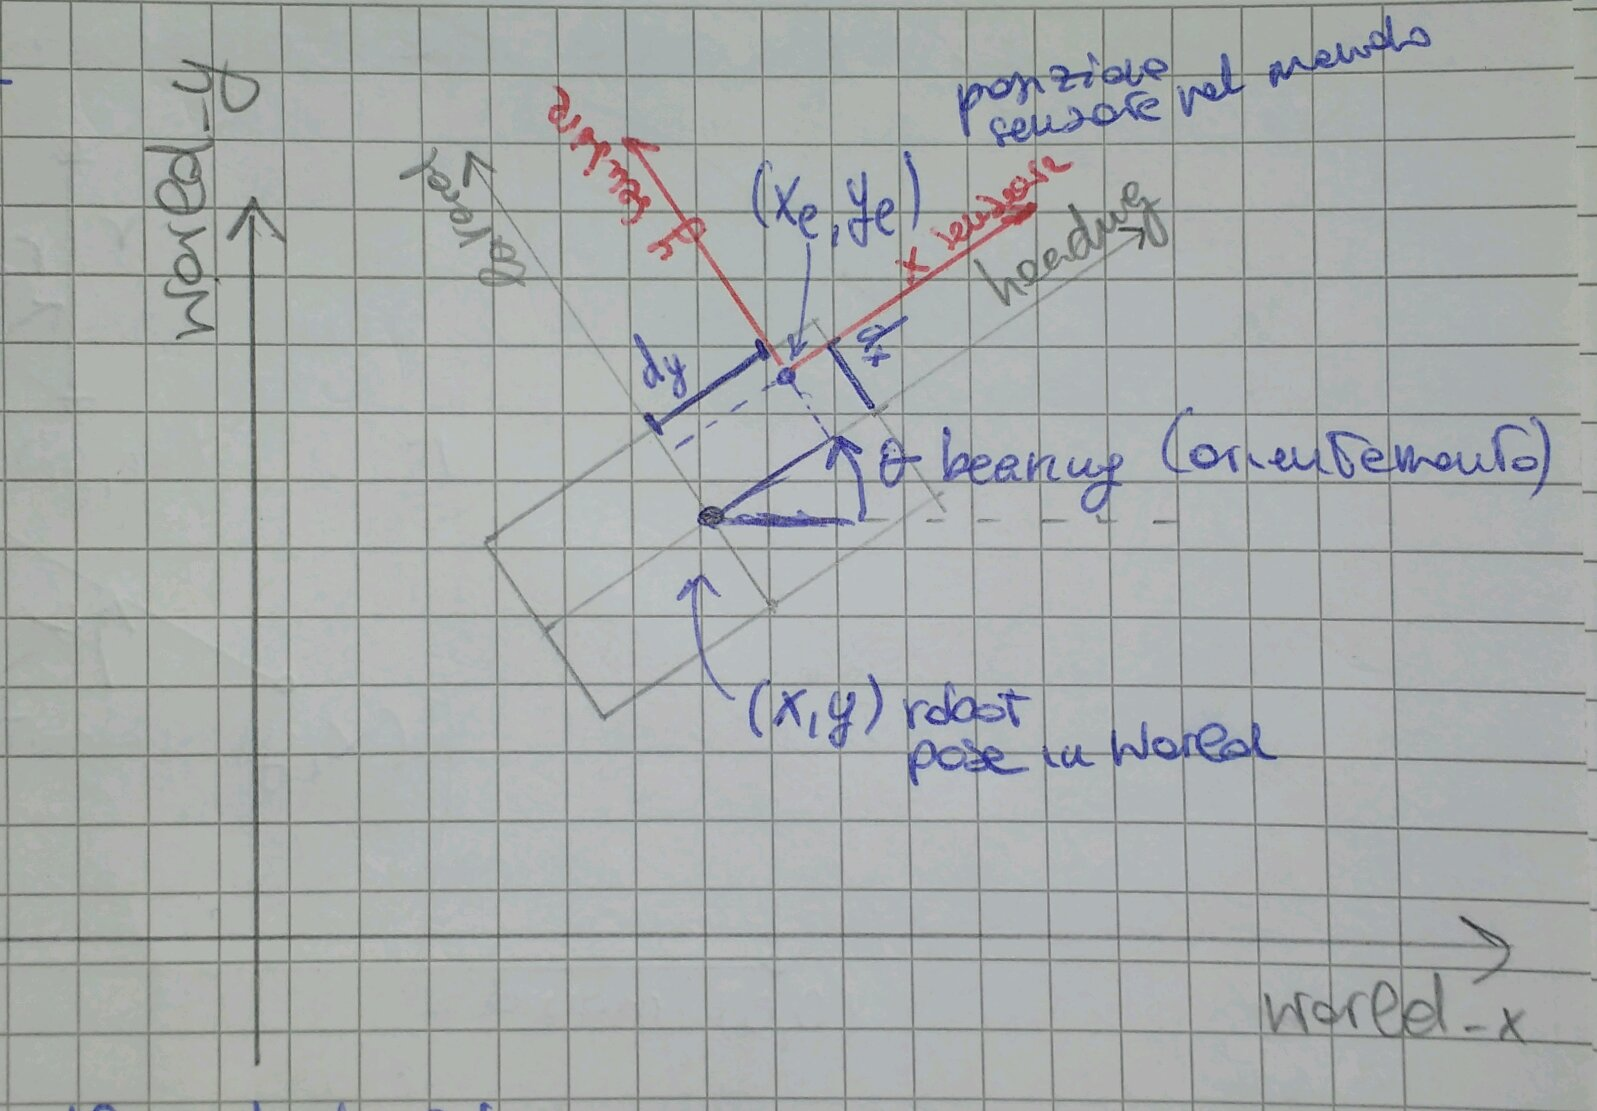
\includegraphics[width=\linewidth]{./img/frames_of_reference.png}
		\caption{The \emph{sensor} \FoR{}, inside the \emph{robot} \FoR{}, inside the \emph{map} \FoR{}.}
		\label{fig.fors.nested}
	\end{subfigure}
	\hfill
	\begin{subfigure}[b]{.38\textwidth}
		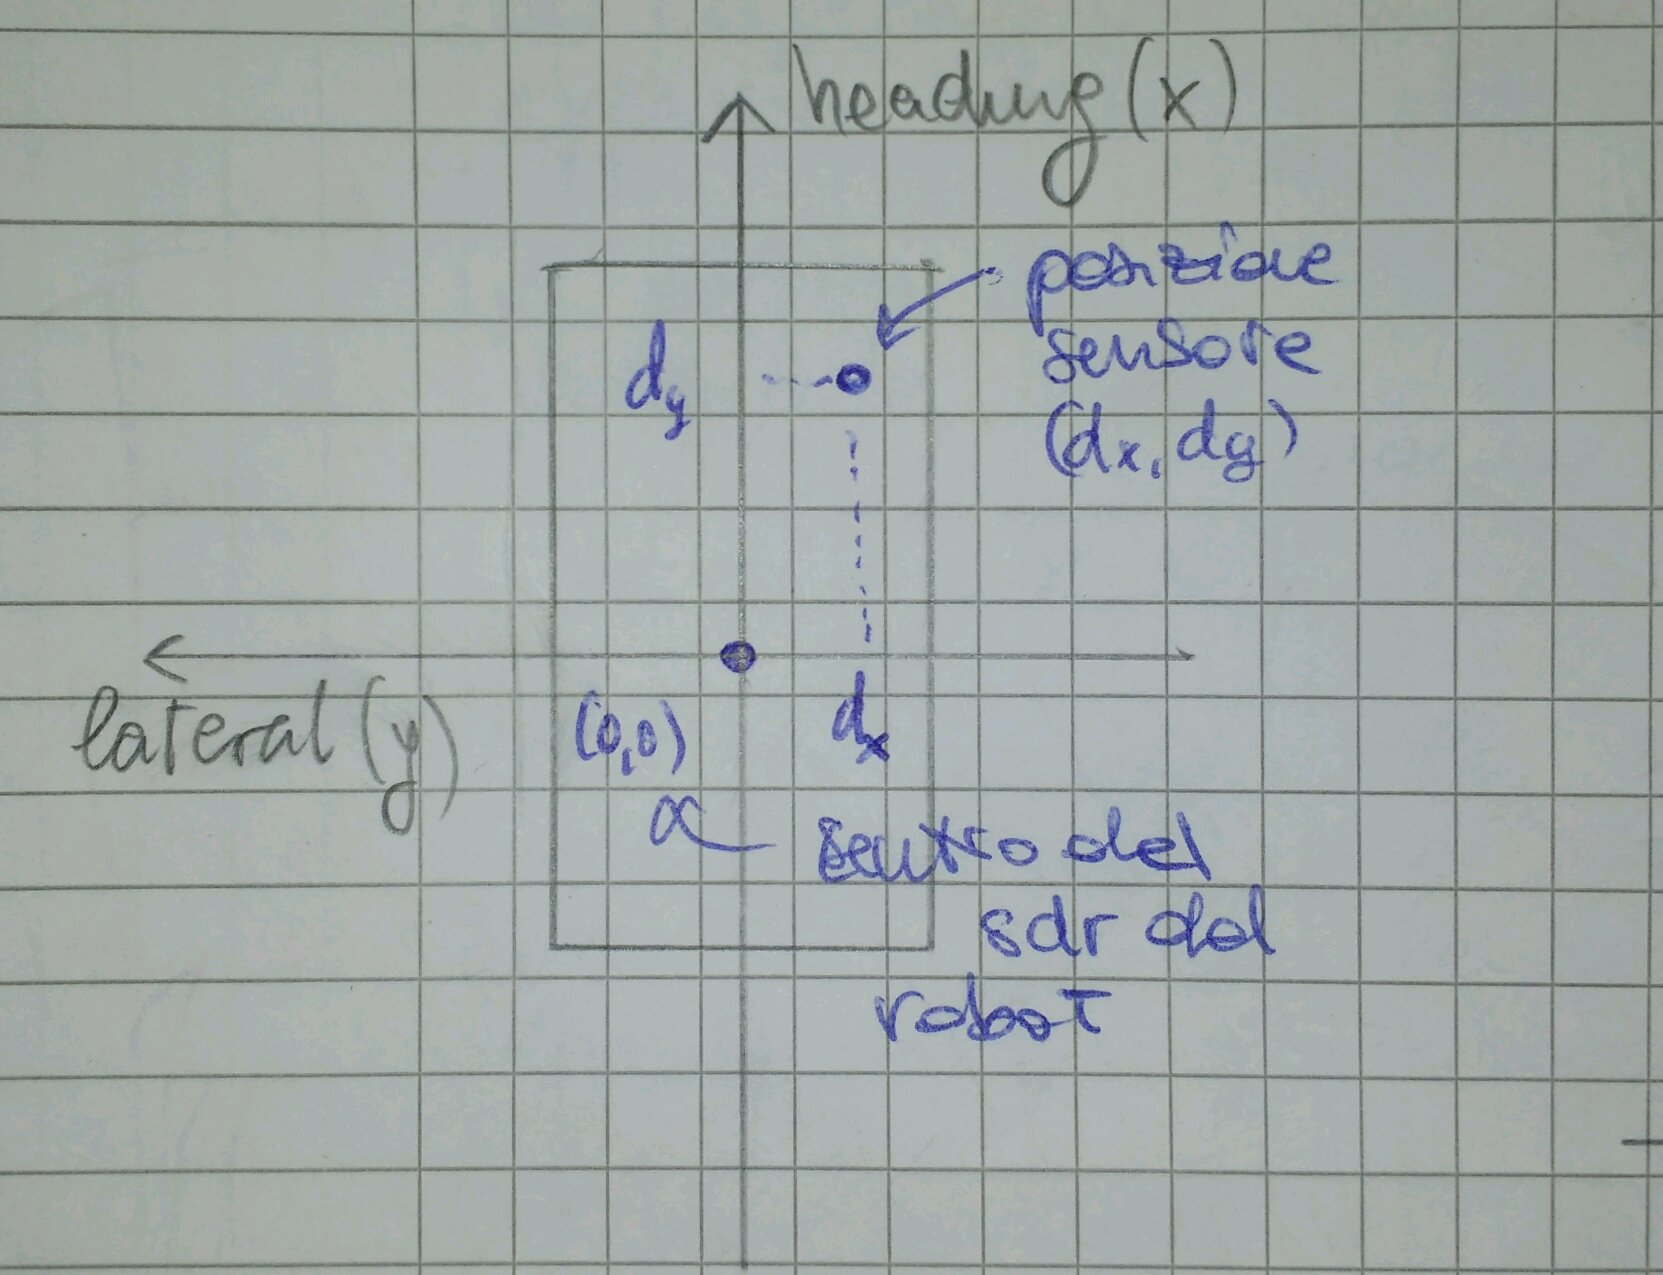
\includegraphics[width=\linewidth]{./img/robot_for.png}
		\caption{The \emph{robot} \FoR{} and the sensor position within it.}
		\label{fig.fors.robot}
	\end{subfigure}
	\caption{Frames of references (\FoR) considered the SLAM problem.}
	\label{fig.fors}
\end{figure}

It is important to understand that several Frames of Reference (\FoR{}) are involved in \SLAM{} (as shown in Figure \ref{fig.fors}):
\begin{itemize}
	\item The \emph{map} (or \emph{global}) \FoR{}, \ie{} the one used for representing the map and the current robot orientation and position. 
	It is arbitrary.
	
	\item The \emph{robot} (or \emph{local}) \FoR{}, \ie{} the one defined according to the reference center of the robot. 
	For what concerns this report, we consider a frame having its origin into the robot geometry center, the abscissas axis always coinciding with the heading direction, and the ordinate axis coinciding with the lateral direction (increasing on the left, as shown in Figure \ref{fig.fors.robot}).
	
	\item The \emph{sensor} (or \emph{measurement}) \FoR{}, which depends on the exteroceptive sensor position within the robot frame, and is in general different from the robot frame. 
	E.g., the sensor may be in position $(d_x,\, d_y)^\top$ w.r.t. the robot frame, as shown in Figure \ref{fig.fors.robot}, and this translation should be taken into account when handling sensor data in order to understand obstacles position on the map.
	In this tutorial we consider, for simplicity, the sensor frame to be coincident with the robot frame \ie{} $d_x = d_y = 0$.
	
\end{itemize}

Please note that, since part of the SLAM process is to build a map of the environment under the hypothesis that the robot has no prior knowledge about it, there is no constraint on how the robot should choose the initial global frame.
In what follows, we (and the robot) assume that the global frame coincides with the initial robot frame, \ie{} the map frame is defined by the initial pose of the robot into the environment: the origin is its \emph{very first} position, the abscissas axis is its \emph{initial} heading direction and, consequently, the ordinate axis is its \emph{initial} lateral direction.

\subsection{The motion model}
	The motion model is a function $g : \mathbb{R}^n \times \mathbb{R}^m \rightarrow \mathbb{R}^n$ mapping the previous robot pose vector, $\vect{r}_{t-1} \in \mathbb{R}^n$, \ie{} the vector containing the robot position and orientation (which are relative to the \emph{map} frame), into the current one, $\vect{r}_t \in \mathbb{R}^n$, by taking into account the last \emph{control} vector $\vect{u}_t \in \mathbb{R}^m$, \ie{} the vector containing proprioceptive data (which is relative to the \emph{robot} frame). More formally:
	\[
		\vect{r}_t = g(\vect{r}_{t-1},\, \vect{u}_t)
	\]
	
	
	
	\paragraph{Example: Differential robot on the plane.}
		Suppose we only own a two-wheeled, differential robot having no odometric sensor, which is often the case in experimental setups. 
	